\chapter{Theoretical Background}
\pagestyle{fancy}
\pagenumbering{arabic}
\section{Standard Model of Particle Physics}

Unless cited otherwise, this section is mostly based on the ``Introduction to elementary particle physics'' by David Griffiths~\cite{griffiths}.

\subsection{General Overview}
\label{sec:stdmdloverview}

The ``Standard Model of particle physics'' that has mostly been developed throughout the last century serves as the basis for almost all analyses in high energy particle physics. It achieves to describe and predict all processes that have been observed with very high precision. The particles, although by themselves very tiny in size ($< 10^{-18}\,\text{m}$), are what our entire (visible) universe consists of. The interactions between these particles are what fuels our sun, transports its energy towards us and keeps us from disintegrating at a nuclear level.


As one is looking for new physics beyond the Standard Model, it is essential to understand said model very well to differentiate between what one perceives as a known process and what goes beyond.

\begin{figure}[ht!]
  \centering
    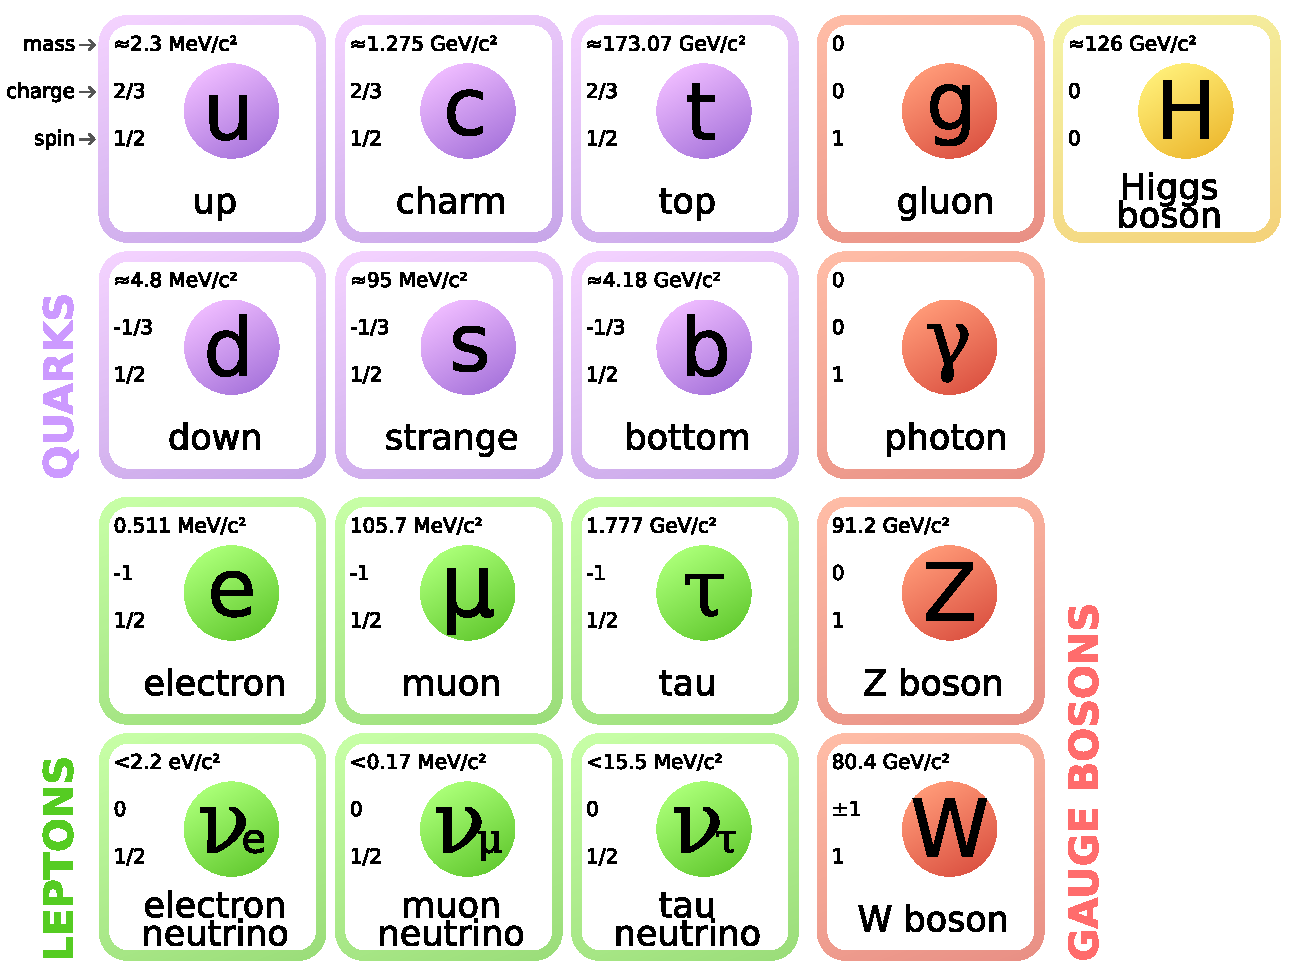
\includegraphics[width=0.9\textwidth]{plots/Standard_Model_of_Elementary_Particles.pdf}
  \caption{The Standard Model's particle content including the latest values~\cite{stdmdlparticles,pdg}.}
  \label{fig:standardmodel}
\end{figure}

\noindent The current ``particle-zoo'', as people like to call the collection of the Standard Model's components, divides all particles into two groups by sorting them based on their spin attribute. The ones with half integer spin are called fermions, while the ones with integer spin are called bosons. The fermion subgroup is once again divided into leptons and quarks, which are grouped into three families each.

Each \textbf{lepton} family is a doublet consisting of a charged $( l, Q_e = -1 )$ and a neutral particle $( \nu_l, Q_e = 0 )$. The doublets have the following particle content:

\begin{equation*}
  \begin{pmatrix}
    \nu_e \\
    e
  \end{pmatrix}
  \quad , \quad
  \begin{pmatrix}
    \nu_\mu \\
    \mu
  \end{pmatrix}
  \quad , \quad
  \begin{pmatrix}
    \nu_\tau \\
    \tau
  \end{pmatrix}
\end{equation*}

The first family is home to the most famous component of the Standard Model, the electron $e$. It is accompanied by the electron neutrino $\nu_e$. Every subsequent family consists of members with the same properties, except for their higher mass. They are named muons $\mu$ and muon neutrinos $\nu_\mu$, as well as taus $\tau$ and tau neutrinos $\nu_\tau$. Due to the mass hierarchy, particles from the higher families usually decay into one of the lower ones, for example $\mu \rightarrow e + \bar{\nu}_e + \nu_\mu$. The main difference between the partner particles of every family, aside from their charge, is the way their interact with matter. While electrons interact with almost anything on a very regular basis, neutrinos are barely noticeable due to their seldom interactions and have gone undetected for more than 20 years after their existence has been proposed.

\textbf{Quarks} do not harbour such fundamental differences between each other. Each family consists of an up-type $( q_u, Q_e = -\frac{2}{3} )$ and a down-type $( q_d, Q_e = +\frac{1}{3} )$ particle. 

\begin{equation*}
  \begin{pmatrix}
    u \\
    d
  \end{pmatrix}
  \quad , \quad
  \begin{pmatrix}
    s \\
    c
  \end{pmatrix}
  \quad , \quad
  \begin{pmatrix}
    t \\
    b
  \end{pmatrix}
\end{equation*}

The first family has the up- and down-flavoured quarks $u$ and $d$, respectively. Similarly to the lepton families, every subsequent family differs only by their increasing mass. Their names are strange $s$ and charm $c$, as well as top $t$ and bottom $b$. Decays like $(udd) \rightarrow (uud) + e + \bar{\nu}_e$ from a higher family to a lower one are also possible. Quarks, as opposed to leptons, cannot be observed in a free state. They are always found in bound states which consist of two or three quarks, which are named mesons and baryons. While the two-quark states are unstable, certain baryons such as the proton $(uud)$ and neutron $(udd)$ are stable over longer periods of time.


While baryons and leptons can join to create atoms and therefore matter, \textbf{bosons} are necessary for the interactions between said particles. Each of the five bosons is responsible for mediating one type of force.

\begin{figure}
  \centering
  \begin{tabular}{ | l | l | c | c | }
    \hline
    Force               & Mediator              & Relative Strength     & Range [m] \\ \hline
    Strong              & Gluons $g$            & $10$                  & $10^{-15}$  \\
    Electromagnetic     & Photons $\gamma$      & $10^{-2}$              & $\infty$  \\
    Weak                & $W$ \& $Z$ bosons     & $10^{-13}$             & $10^{-18}$  \\
    Gravitation         & Graviton $G$          & $10^{-42}$             & $\infty$  \\
    \hline  
  \end{tabular}
  \caption{The four fundamental forces and their attributes. ``Strength'' is to be taken as a rough estimate, as it ultimately is an ambiguous quantity. It depends on the nature of the source and what it is applied on.}
  \label{tab:fundforces}
\end{figure}

For electromagnetic interactions, such as electron pair production and annihilation $e^+ e^- \rightarrow \gamma \rightarrow e^+ e^-$, the photon $\gamma$ is the mediator. The strong force's gluons $g$ mediate interactions between quarks. They are able to bind quarks (e.g. of a proton) despite the electromagnetic repulsion, due to it being a 100 times stronger at that scale. The weak force is mediated by the two vector bosons $W$ and $Z$. Unlike the other forces, the weak one is able to change the flavour of quarks (even violating the otherwise conserved family number) and leptons. Gravitons $G$ have been predicted, but not yet observed. Gravitation is the only fundamental force with a long range, which does not have a repulsive component, as there are no negative masses. Along with its infinite range, it therefore dominates on large, cosmic scales and is responsible for the formation of galaxies and their substructures. Since there is no quantized formulation of the gravitational force, it is not part of the Standard Model.


For every particle there is also a corresponding antiparticle. Antiparticles have the same properties as their normal counterparts, except for their charge-like properties. For example a negatively charged electron $(Q_e = -1)$ has a positively charged $(Q_e = +1)$ antiparticle called the positron. For uncharged particles, this means that they are their own antiparticle. Collisions between a particle and its counterpart usually leads to ``annihilation''. As the name suggests, this leads to both objects being destroyed. Particles produced in this annihilation carry the energy, which is set free in the process. Taking the electron-positron annihilation as an example, the resulting photon can also produce matter once again, it has enough energy. At least the rest mass of both particles in terms of energy is necessary. This means for the aforementioned example that an electron-positron production (``pair production'') is possible, but not necessarily the only option. Similarly muons, taus or quarks could have been the result as long as the charge-like properties are being conserved in the process.


\subsection{Gauge Symmetry}

The Standard Model of particle physics is a relativistic gauge theory, which is invariant under local gauge transformations. Similarly to the Euler-Lagrange approach to classical mechanics

\begin{equation}
  \label{eq:eulerlagrange}
  \frac{d}{dt} \left( \frac{\partial L}{\partial \dot{q}_i} \right) =  \frac{\partial L}{\partial q_i} \quad \text{with } L = T - U,
\end{equation}

\noindent relativistic field theories are formulated using a Lagrangian (density) $\mathcal{L} ( \phi_i, \partial_\mu \phi_i )$, which is a function of time and spatial coordinates as well as its derivatives. It is a necessary transition from a classical particle to a quantized object. The equation using this Langrangian has the following shape.

\begin{equation}
  \label{eq:lagrangian}
  \partial_\mu \left( \frac{\partial \mathcal{L}}{\partial (\partial_\mu \phi_i)} \right) = \frac{\partial \mathcal{L}}{\partial \phi_i} \quad (i = 1, 2, 3, 4)
\end{equation}

Further studies using this equation have lead to the formulation of the weak, strong and electromagnetic force as gauge theories. 

\subsection{Local Gauge Invariance}

The most basic Lagrangian for a spin $\frac{1}{2}$ particle is called a ``Dirac Lagrangian''. It describes a free particle with no external fields:

\begin{equation}
  \label{eq:diraclagrangian}
  \mathcal{L} = i (\hbar c) \bar{\psi} \gamma^\mu \partial_\mu \psi - (m c^2) \bar{\psi} \psi
\end{equation}

\noindent Here the $\psi$ are called ``Spinors'' and are the most basic description of a particle. One can see that under a global gauge transformation, similarly to adding a phase,

\begin{equation}
  \label{eq:globalgaugeinv}
  \psi \rightarrow e^{i \theta} \psi
\end{equation}

\noindent the equation remains invariant. The sign of the exponent will change with complex conjugation and both exponential functions will cancel each other out. Considering that physics should not depend on the location (disregarding external factors), requiring local gauge invariance is necessary:

\begin{equation}
  \label{eq:localgaugeinv}
  \psi \rightarrow e^{i \theta(x)} \psi
\end{equation}

\noindent Doing so will however yield additional terms stemming from the derivation of $e^{i \theta(x)}$ which need to be dealt with. 

\subsection{Quantum Electro Dynamics}
\label{sec:qed}

To compensate for the terms added by requiring local gauge invariance, the covariant derivation is introduced:

\begin{align}
  \label{eq:covariantderivative}
  \mathcal{D}_\mu = \partial_\mu + i \frac{q}{\hbar c} A_\mu
\end{align}

\noindent Using equation~(\ref{eq:covariantderivative}), the invariance of the Lagrangian is restored, but it also adds a spin-1 vector field $A_\mu$, which requires its own additional terms. The basic Lagrangian for such a field is given by:

\begin{equation}
  \label{eq:procalagrangian}
  \mathcal{L} = - \frac{1}{16 \pi} F^{\mu \nu} F_{\mu \nu} + \frac{1}{8 \pi} \left( \frac{m_A c}{\hbar} \right)^2 A^\nu A_\nu - \frac{1}{c} \underbrace{J^\mu}_{Source} A_\mu \quad \text{with } F^{\mu \nu} = \partial^\mu A^\nu - \partial^\nu A^\mu
\end{equation}

\noindent While the first and the last term are locally gauge invariant, the middle one is not. This necessitates a massless mediator $m_A = 0$ to conserve the invariance. Adding both components of the Lagrangians results in

\begin{equation}
  \label{eq:qedlagrangian}
  \mathcal{L}_{\text{QED}} = i (\hbar c) \bar{\psi} \gamma^\mu \partial_\mu \psi - (m c^2) \bar{\psi} \psi - \frac{1}{16 \pi} F^{\mu \nu} F_{\mu \nu} - \frac{1}{c} \underbrace{J^\mu}_{Source} A_\mu,
\end{equation}

\noindent which is the Lagrangian for quantum electro dynamics. So by requiring local gauge invariance under a transformation $\psi \rightarrow U \psi$ with a unitary $1 \times 1$ matrix $U$, here $U = e^{i \theta}$, the photon as the mediator of the electromagnetic force is introduced to the free Lagrangian. It is massless, has a spin of 1 and since its transformation does commutate, it does not interact with other photons. The latter aspect is also coherent with the photon not carrying any charge. The group of all such transformations is called $U(1)$. Using the same principle but different groups of transformations, the remaining interactions will be introduced as well.

\subsection{Quantum Chromo Dynamics}
\label{sec:qcd}

Expanding local gauge invariance from unitary $1 \times 1$ transformations $U(1)$ to the special unitary group $SU(3) = U(1) \otimes U(3)$, one adds the strong interaction to the Lagrangian. The generators of the $SU(3)$ $T_a$ can be described using the Gell-Mann matrices $\lambda_a$ using the relation $T_a = \lambda_a / 2$ with $a = 1, ..., 8$. The important difference between these two groups of transformations is that the $SU(3)$ is not abelian, but adheres the commutation relations given by

\begin{equation}
  \label{eq:qcdgencommute}
  \left[ T_a, T_b \right] = i \sum_{c=1}^8 f_{abc} T_c,
\end{equation}

\noindent where $f_{abc}$ is the structure constant of the $SU(3)$. The previously single component spinors $\psi$ now carry the colour charge and are extended as follows:

\begin{equation}
  \label{eq:colorspinor}
  \psi \rightarrow \psi = \begin{pmatrix}
    \psi_r \\
    \psi_g \\
    \psi_b
  \end{pmatrix}
\end{equation}

\noindent Requiring local gauge invariance results once again in new gauge fields, similarly to QED (Sec.~\ref{sec:qed}). These 8 new fields correspond their respective gluons. Since the transformation is not abelian, these mediators self-couple. This means that they carry a colour charge. The reason for the naming scheme being borrowed from chromatics, is due to the way particles couple. You can only observe colour neutral states. This means that a quark, which are the only fermions to carry a colour charge in the Standard Model, has two options. Either couple to a quark of its anticolour or two other quarks, who carry the remaining two colour charges of the $r,g,b$ triplet. Keeping the titles from section~\ref{sec:stdmdloverview} in mind, those are called mesons and baryons respectively.

Another important aspect of QCD that stems from the self-coupling of gluons, is the behaviour of the strong coupling constant $\alpha_s(Q^2)$. Since it decreases as function of rising momentum transfer $Q^2$, the particles become less constrained the higher the energy scale of the interaction. This is called ``asymptotic freedom'' and can be described pertubatively. On the other end of the scale, around $\sqrt{Q^2} \sim 200\,\text{MeV}$, $\alpha_s{Q^2}$ becomes very large and this freedom turns into ``confinement''. Here the pertubation theory diverges and quarks as well as gluons do not appear as free particles anymore.

\subsection{Electro Weak Theory}

Unlike both the electromagnetic and strong interaction, the weak force has two different ``types'' of interactions. The neutral current (NC) interactions are mediated by the $Z$-boson and behave very similarly to the ones based on an exchange of photons $\gamma$. Charged current (CC) interactions have $W^\pm$ as their gauge boson and contrary to all other types of interactions, it allows for changes of flavour.

Historically, the discovery of the charged currents precedes the one of neutral ones. To describe it as a gauge theory, the symmetry group $SU(2)_L$ is being used. The index ``L'' indicates that these types of currents only couple to left-handed and therefore violates parity conservation maximally. In reference to the spin and isospin attributes, the charge of this interaction is called ``weak isospin'' $I^3$. Using the weak isospin, left-handed particles can be sorted into doublets with $e^-_L$ and $u_L$ having $(I = \frac{1}{2}, I^3 = -\frac{1}{2})$, as well as $\nu_L$ and $d_L$ having $(I = \frac{1}{2}, I^3 = +\frac{1}{2})$. Since right-handed particles do not partake in the charged current interaction, they are sorted into singlets with $(I = 0, I^3 = 0)$.


Using the $SU(2)_L$ symmetry group, yields a third weak interaction. As this still only couples to left-handed particles, it cannot be the weak neutral current which couples to both types. Instead a generator called ``hypercharge'' $Y$ is introduced and defined by:

\begin{align}
  \label{eq:hypercharge}
                  Q_e &= I^3 + \frac{Y}{2} \\
  \Leftrightarrow Y   &= 2 \left( Q_e - I^3 \right)
\end{align}

\noindent This extends the symmetry group by a $U(1)_Y$, thus being $SU(2)_L \otimes U(1)_Y$. The resulting gauge fields are called $W^i_\mu, i = 1,2,3$ for the $SU(2)_L$ and $B_\mu$ for the $U(1)_Y$. These gauge fields mix into two charged and two neutral bosons:

\begin{align}
  \label{eq:ewbosons}
  W^\pm_\mu & = \sqrt{\frac{1}{2}} \left( W^1_\mu \mp W^2_\mu \right) \\
  A_\mu & = \ B_\mu \cos{\theta_W} + W^3_\mu \sin{\theta_W} \\
  Z_\mu & = - B_\mu \sin{\theta_W} + W^3_\mu \cos{\theta_W}
\end{align}
 
\noindent The mixing-angle $\theta_W$ is a free parameter of the Standard Model, meaning that it cannot be predicted from its theoretical construct and has to be measured instead. While the $W^\pm$ and $Z$ bosons are represented by their respective fields, $A_\mu$ can be recognized as the photon introduced in QED (Sec.~\ref{sec:qed}). The electroweak theory therefore describes the combination of both the electromagnetic and weak interaction by unifying them into a single gauge theory.


The Standard Model of particle physics describes nature very well. One of the most precise measurements (and tests of QED), is the ``g-factor'' of the electron's magnetic momentum. While the agreement between theory and experiment can be as good as multiple orders of magnitude as in the aforementioned case, there are still certain discrepancies between theory and experiment in the Standard Model. One of them will be addressed in the following section.

\subsection{The Higgs Mechanism}
\label{sec:higgs}

While the initial two mediators of the respective gauge theories were massless, the $W$ and $Z$ bosons are not. In fact, they are quite heavy with roughly $80.4\,\text{GeV}$ for the $W$ and $90.2\,\text{GeV}$ for the $Z$. This means that the mass terms for both bosons do not vanish and therefore the local gauge invariance, as described in the QED section (Sec.~\ref{sec:qed}), is violated. To alleviate this issue, the concept of ``spontaneous symmetry breaking'' can be used. For this purpose a new field is introduced to the Lagrangian:

\begin{equation}
  \label{eq:higgslagrangian}
  \mathcal{L} =  \frac{1}{2} (\partial_\mu H)^* (\partial^\mu H)  + \frac{1}{2} \mu^2 (H^* H) - \frac{1}{4} \lambda^2 (H^* H)^2
\end{equation}

\noindent Unlike the spinors used in the previous equations, the field $H$ is imaginary and scalar.

\begin{equation}
  \label{eq:higgsimfield}
  H = H_1 + i H_2.
\end{equation}

\noindent While spatial symmetry $H \rightarrow - H$ is maintained, the same cannot be said for the ground state anymore. As shown in figure~\ref{fig:higgspotential}, a unique, non-symmetrical ground state can be attained through spontaneous symmetry breaking.


\begin{figure}[ht!]
  \centering
    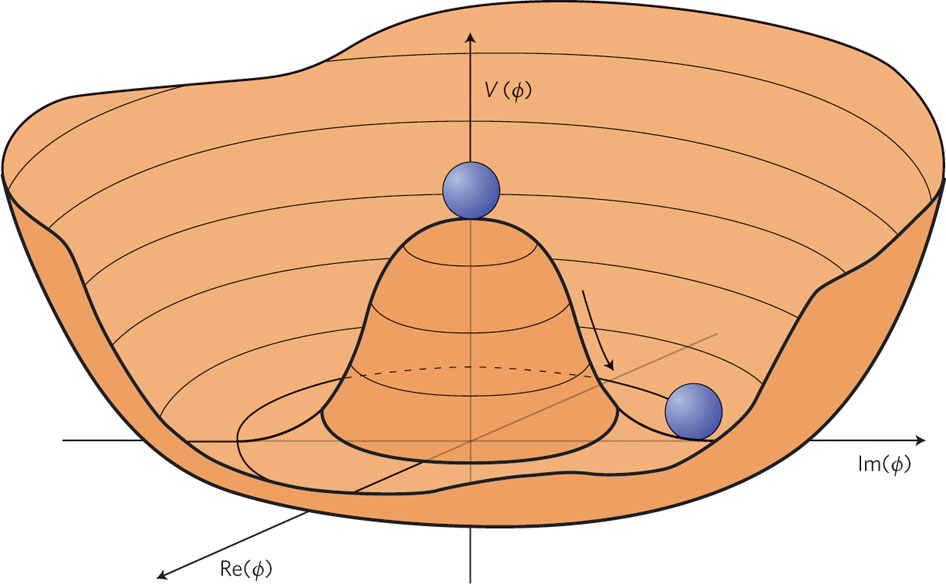
\includegraphics[width=0.5\textwidth]{plots/higgspotential.jpg}
  \caption{The potential of the Higgs-Lagrangian. It is shown how through spontaneous symmetry breaking a non-symmetric ground state can be chosen~\cite{higgspotential}.}
  \label{fig:higgspotential}
\end{figure}


This extension to the theory described by the Lagrangian was suggested by Peter Higgs, who also lends his name to the ``Higgs-boson''. The masses of particles depend on their coupling to the Higgs-field. The stronger the coupling, the higher the mass. As the Higgs-boson also couples to itself, it is massive, too.

The search for the Higgs boson by the CMS collaboration at the Large Hadron Collider has found statistically significant evidence for the existence of a new boson (which resembles the proposed Higgs boson very closely). While previous publications have already shown a $5 \sigma$ excess around the invariant mass of $m_X = 125\,\text{GeV}$~\cite{higgscls}, further studies have been performed on the $H \rightarrow ZZ$ decay mode. Taken from their publication of the 29th of December in 2012, one can see the invariant mass of four selected leptons $m_{4 l}$ in figure~\ref{fig:higgsmzz}.

\begin{figure}[ht!]
  \centering
    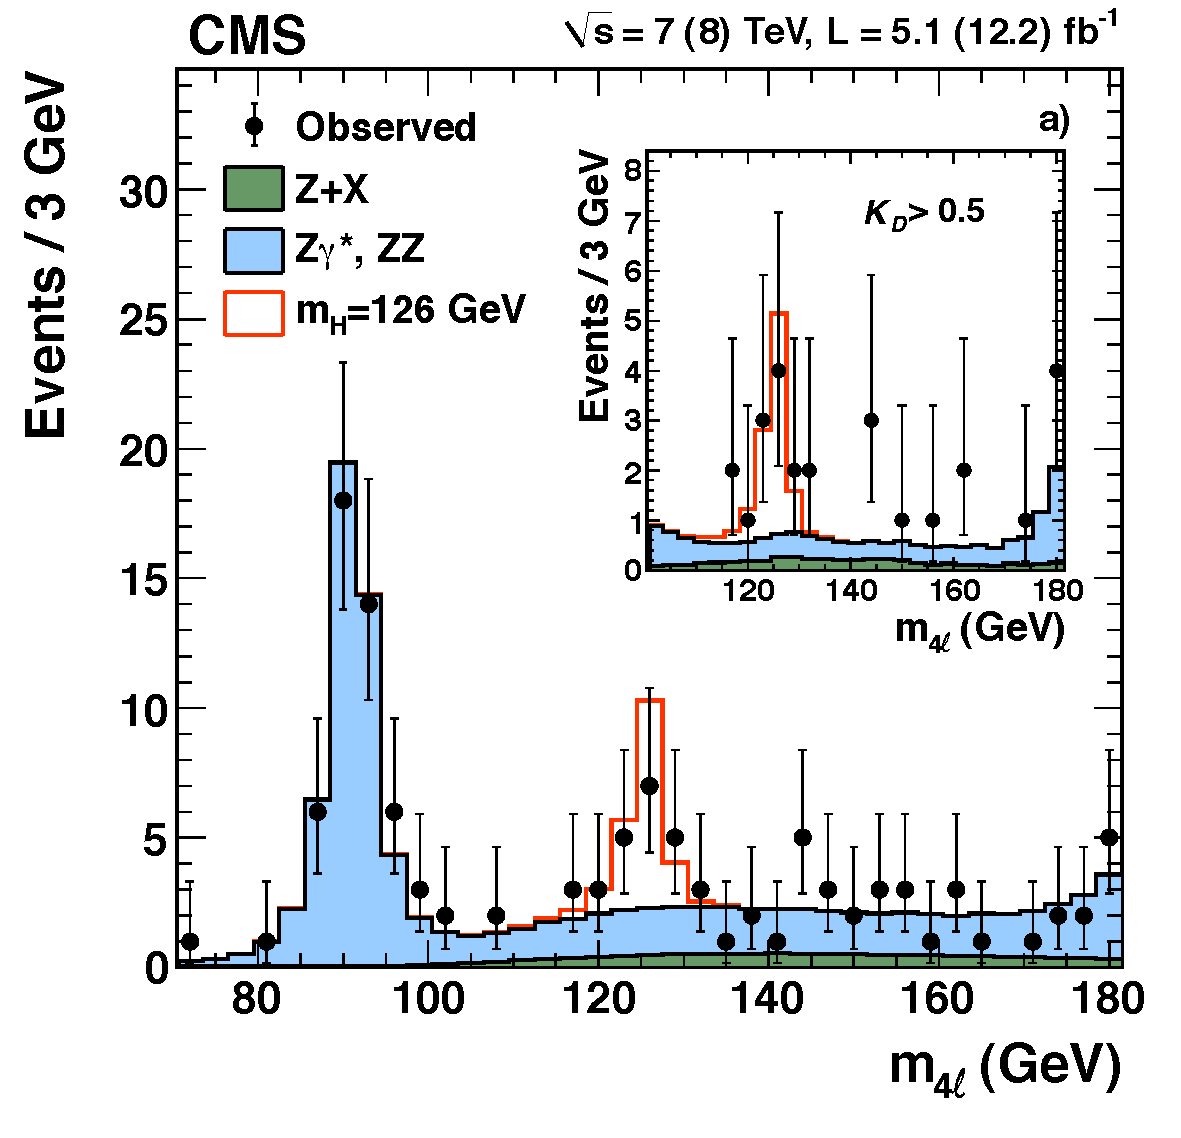
\includegraphics[width=0.6\textwidth]{plots/higgsmzz.pdf}
  \caption{Invariant mass of 4 leptons around the $125\,\text{GeV}$ area, where an excess was observed beforehand~\cite{higgsmzz}.}
  \label{fig:higgsmzz}
\end{figure}

\noindent Combining the results from the $H \rightarrow ZZ$ decay channel with the $H \rightarrow \gamma \gamma$ one, which are the two channels with the best mass resolution, yields the current best mass estimate of $125.8 \pm 0.4 \,\text{(stat)} \pm 0.4\,\text{(syst)}\,\text{GeV}$~\cite{higgsmzz}.


%%% Local Variables: 
%%% mode: latex
%%% TeX-master: "document"
%%% End: 
